\documentclass[11pt]{article}
\usepackage[margin=1in]{geometry}
\usepackage{amsmath,amssymb}
\usepackage{graphicx}
\usepackage{hyperref}

\title{Multiwavelength Observations, Spectral Energy Distributions, and Variability of Blazars}
\author{Suryapriya CS}
\date{8th August 2026}

\begin{document}
\maketitle

\begin{abstract}
\noindent
Active galactic nuclei (AGN) hosting relativistic jets aligned closely with the observer's line of sight --- collectively classified as blazars --- represent some of the most luminous, energetic, and variable non-explosive phenomena known in the universe. Powered by accretion onto supermassive black holes with masses spanning $M_{\mathrm{BH}} \sim 10^{6}$--$10^{10}\,M_{\odot}$, blazars are distinguished from other radio-loud AGN by the extreme relativistic beaming that occurs when a jet is oriented within a few degrees of the line of sight, amplifying both observed flux and variability across the entire electromagnetic spectrum. This review synthesizes the current observational and theoretical understanding of blazar astrophysics, drawing on multiwavelength observational campaigns, high-redshift surveys, long-term variability studies, and theoretical emission modeling.

We first summarize the structural and classification framework of AGN and blazars, distinguishing Flat Spectrum Radio Quasars (FSRQs) and BL Lacertae (BL Lac) objects on the basis of optical emission-line strength and radiative efficiency, and situating both within the Low-, Intermediate-, and High-Synchrotron-Peaked (LSP/ISP/HSP) sequence defined by the frequency of the synchrotron spectral peak. Particular attention is given to the physical basis of the observed inverse relationship between synchrotron peak frequency and Compton dominance, which links jet power, accretion regime, and radiative mechanism across the blazar population.

The review then surveys multiwavelength observations band by band --- radio, infrared, optical, ultraviolet, X-ray, and gamma-ray --- highlighting the distinct physical components each waveband probes, from VLBI-resolved superluminal jet motions and radio-band opacity effects, through thermal accretion-disk and torus signatures in the infrared--optical--ultraviolet, to the diagnostic power of X-ray and gamma-ray data in tracing the rising and falling edges of the high-energy spectral hump. These multiwavelength diagnostics are synthesized within the framework of the broadband spectral energy distribution (SED), whose characteristic double-humped shape is interpreted through synchrotron and inverse-Compton radiative processes. We discuss both leptonic emission scenarios --- Synchrotron Self-Compton (SSC), dominant in BL Lac objects, and External Compton (EC) scattering of disk, broad-line region, or dusty-torus photons, dominant in FSRQs --- and hadronic scenarios involving proton synchrotron and photohadronic cascade emission, weighing their respective successes and energetic limitations.

Variability phenomenology is examined across timescales ranging from minutes to decades, encompassing intraday very-high-energy flares that demand extremely compact emission regions and high Doppler factors, as well as long-term statistical behavior including the redder-when-brighter spectral trend, fractional variability differences between FSRQs and BL Lacs, power spectral density and flux-distribution statistics, and candidate quasi-periodic oscillations whose statistical significance remains contested. We further review the emerging role of multi-messenger astronomy, including the landmark coincidence between a high-energy IceCube neutrino and a flare from TXS~0506+056 as direct evidence for hadronic acceleration, alongside the more speculative but rapidly developing prospects for gravitational-wave connections to blazar activity.

Finally, we outline the principal open challenges confronting the field --- most notably the unresolved location of the gamma-ray dissipation region and the physical origin of GeV spectral breaks in luminous FSRQs --- and discuss how forthcoming facilities, including the Cherenkov Telescope Array, X-ray and gamma-ray polarimetry, next-generation VLBI networks, and expanded neutrino and gravitational-wave observatories, are poised to resolve these questions and further establish blazars as premier laboratories for relativistic jet physics and black hole accretion.

\noindent\textbf{Keywords:} active galactic nuclei; blazars; relativistic jets; spectral energy distributions; multiwavelength astronomy; variability; multi-messenger astrophysics
\end{abstract}

\newpage

%%%%%%%%%%%%%%%%%%%%%%%%%%%%%%%%%%%%%%%%%%%%%%%%%%%%%%
\section{Introduction}

Blazars constitute an extreme subclass of radio-loud Active Galactic Nuclei (AGN), powered by accretion onto supermassive black holes with masses in the range $M_{\mathrm{BH}} \sim 10^{6}$--$10^{10}\,M_{\odot}$, situated at the centers of their host galaxies \cite{Kormendy2013,Urry1995}. When an AGN launches a highly collimated relativistic jet oriented within a small angle ($\theta \lesssim 5^{\circ}$) of Earth's line of sight, relativistic beaming substantially amplifies both the observed flux and its variability across nearly every accessible waveband --- from radio wavelengths through high-energy (HE, $E>100\,\mathrm{MeV}$) and very-high-energy (VHE, $E>100\,\mathrm{GeV}$) gamma rays \cite{Urry1995,Blandford1978}. Advances in multiwavelength instrumentation --- including the \textit{Fermi}-LAT, \textit{Swift}, and \textit{NuSTAR} space observatories, together with ground-based radio, optical, near-infrared (NIR), and Imaging Atmospheric Cherenkov Telescope (IACT) facilities such as H.E.S.S., MAGIC, and VERITAS --- have substantially advanced our understanding of jet energetics, particle acceleration mechanisms, and the interplay between relativistic jets and their accretion disks \cite{Atwood2009,Gehrels2004,Harrison2013,Hinton2004,Holder2006,Aleksic2016}.

\begin{figure}[htbp]
\centering
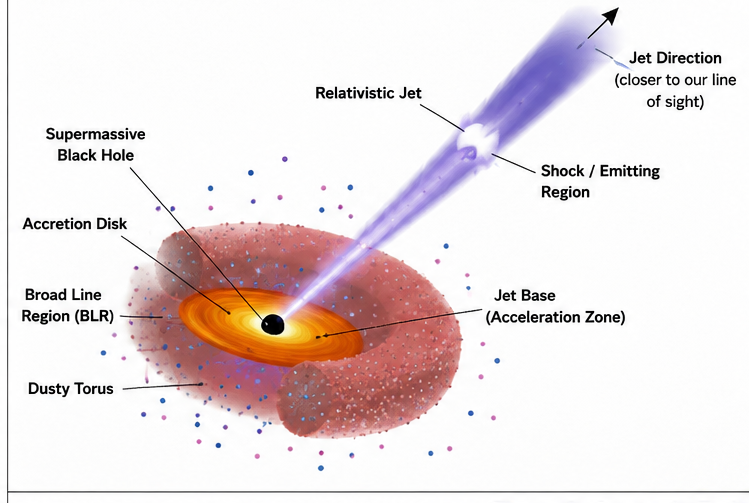
\includegraphics[width=0.75\textwidth]{fig1_blazar_agn.png}
\caption{Unified AGN orientation scheme. A single population of radio-loud AGN, viewed at different angles to a common relativistic jet axis, produces the observed diversity of blazars, quasars, and radio galaxies: at small viewing angles ($\theta \lesssim 5^{\circ}$) relativistic beaming makes the jet dominate the SED (blazars); at intermediate angles the accretion disk and BLR are more directly visible (FSRQs/quasars); at large angles the source appears as an FR~I/FR~II radio galaxy \cite{Urry1995}.}
\label{fig:agn-unification}
\end{figure}

Figure~\ref{fig:agn-unification} illustrates this orientation-based unification scheme, which underlies the classification framework adopted throughout this review.

%%%%%%%%%%%%%%%%%%%%%%%%%%%%%%%%%%%%%%%%%%%%%%%%%%%%%%
\section{Multiwavelength Observations}

The broadband emission of blazars spans more than twenty decades in photon frequency, from radio wavelengths to very-high-energy (VHE) gamma rays. No single instrument or waveband can capture the full diagnostic power of blazar spectral energy distributions (SEDs); consequently, coordinated multiwavelength (MWL) campaigns combining space- and ground-based facilities have become the standard observational approach. Each waveband probes a distinct physical component of the source --- the jet, the accretion disk, the broad-line region (BLR), or the dusty torus --- and their combined analysis constrains jet kinematics, particle energy distributions, and radiative mechanisms.

\subsection{Radio Observations}

Radio emission from blazars is dominated by optically thick-to-thin synchrotron radiation from relativistic electrons in the jet, producing the characteristically flat or inverted radio spectra ($\alpha \lesssim 0.5$, where $S_\nu \propto \nu^{-\alpha}$) that distinguish blazars from steep-spectrum radio galaxies. Very Long Baseline Interferometry (VLBI) at 15--43~GHz resolves milliarcsecond-scale jet structure and enables direct measurement of apparent superluminal motions ($\beta_{app} > 1$), providing the most direct kinematic evidence for bulk relativistic outflow. Long-term monitoring programs (e.g., the Owens Valley Radio Observatory 40~m and MOJAVE VLBI surveys) reveal that radio flares are frequently associated with the ejection of new superluminal knots from the millimeter-wave core, and that radio variability typically lags high-energy gamma-ray activity by tens to hundreds of days. This lag is attributed to synchrotron self-absorption and opacity effects within the compact, optically thick jet base, implying that the radio-emitting region lies downstream of the primary gamma-ray dissipation site.

\subsection{Infrared Observations}

Infrared (IR) observations trace both the low-frequency tail of jet synchrotron emission and thermal reprocessing by the circumnuclear dusty torus. In flat spectrum radio quasars (FSRQs), NIR photometry (J, H, K bands) is a sensitive tracer of jet activity, since synchrotron emission dominates over any residual thermal contribution at these wavelengths. Long-term NIR/optical monitoring campaigns, such as the decade-long SMARTS program covering dozens of \textit{Fermi}-detected blazars, show that intrinsic variability amplitude in the NIR systematically exceeds that in the optical B band, confirming that redder, non-thermal jet emission dominates the variable component of the SED. Mid-infrared data from facilities such as \textit{WISE} additionally allow separation of the thermal torus bump (peaking near rest-frame $10$--$30~\mu$m) from the non-thermal jet continuum, constraining torus luminosities and dust temperatures ($T_{\text{dust}} \sim 1000$~K) relevant to external Compton emission models.

\subsection{Optical Observations}

Optical observations probe the transition region between jet synchrotron emission and thermal accretion disk radiation. In BL Lac objects, the optical continuum is essentially pure non-thermal jet emission, exhibiting rapid variability and characteristic power-law spectral shapes. In FSRQs, particularly at high redshift ($z > 2.5$), a thermal ``big blue bump'' from the accretion disk is often visible superimposed on the jet continuum, allowing simultaneous constraints on disk luminosity ($L_d \sim 10^{46}$--$10^{47}\,\text{erg s}^{-1}$) and black hole mass ($M_{\text{BH}} \sim 10^{9}\,M_\odot$). Optical polarimetry provides an independent diagnostic of jet magnetic field structure, with rotations in polarization angle often coincident with gamma-ray flaring activity, suggesting a common origin in regions of ordered or turbulent magnetic field associated with propagating shocks or reconnection sites. Long-term optical light curves also reveal the widespread redder-when-brighter (RWB) trend observed in roughly 80\% of monitored blazars.

\subsection{Ultraviolet Observations}

Ultraviolet observations, obtained with instruments such as \textit{Swift}-UVOT and archival \textit{International Ultraviolet Explorer} and \textit{Hubble Space Telescope} data, primarily sample the peak of accretion disk thermal emission in luminous FSRQs, as well as line emission from the broad-line region. UV spectroscopy enables direct measurement of BLR emission-line equivalent widths, the principal criterion distinguishing FSRQs (EW~$>5$~\AA) from BL~Lac objects (EW~$<5$~\AA). In blazars where the disk and BLR are directly detected, UV data anchor estimates of ionizing luminosity and black hole mass via virial or disk-continuum scaling relations, and constrain the seed photon field available for external Compton scattering in the jet.

\subsection{X-ray Observations}

X-ray observations, obtained with \textit{Swift}-XRT \cite{Gehrels2004}, \textit{NuSTAR} \cite{Harrison2013}, \textit{XMM-Newton}, and \textit{Chandra}, sample the transition region between the synchrotron and inverse-Compton components of the SED and are essential for distinguishing blazar subclasses. In high-synchrotron-peaked (HSP) BL Lac objects, X-rays trace the falling edge of the synchrotron hump, while in FSRQs and low-synchrotron-peaked sources, X-rays trace the rising portion of the high-energy inverse-Compton hump. Joint \textit{Swift}-XRT/\textit{Fermi}-LAT campaigns on high-redshift FSRQs typically find hard X-ray photon indices $\Gamma_X \sim 1.0$--$1.9$, consistent with this rising-hump interpretation. X-ray spectral curvature and rapid X-ray variability (on timescales of hours) in HSP sources provide some of the tightest constraints on electron acceleration and cooling timescales in the jet, and X-ray polarimetry from \textit{IXPE} now offers a direct probe of magnetic field ordering in the synchrotron-emitting region.

\subsection{Gamma-ray Observations}

Gamma-ray observations define blazars as a class and constrain the high-energy peak of the SED. \textit{Fermi}-LAT \cite{Atwood2009} has provided nearly two decades of continuous all-sky monitoring in the HE band ($>100$~MeV), enabling systematic variability, spectral, and population studies of thousands of gamma-ray blazars. FSRQs typically exhibit soft HE photon indices ($\Gamma_\gamma \gtrsim 2.2$) and pronounced spectral curvature near a few GeV, while BL Lac objects display harder spectra ($\Gamma_\gamma \lesssim 2.0$) extending to higher energies. At VHE energies ($>100$~GeV), ground-based IACTs (H.E.S.S.\ \cite{Hinton2004}, MAGIC \cite{Aleksic2016}, VERITAS \cite{Holder2006}) have detected dozens of blazars, predominantly HSP BL Lacs, revealing extremely rapid flaring on timescales as short as minutes and requiring the most extreme Doppler factors ($\delta \sim 50$) inferred anywhere in blazar science. The forthcoming Cherenkov Telescope Array (CTA) will substantially extend VHE sensitivity and temporal resolution, improving constraints on both intrinsic jet physics and the intervening extragalactic background light (EBL).

%%%%%%%%%%%%%%%%%%%%%%%%%%%%%%%%%%%%%%%%%%%%%%%%%%%%%%
\section{Spectral Energy Distribution}

The broadband SED of a blazar, plotted as $\log(\nu F_\nu)$ versus $\log \nu$, characteristically displays two smooth, broad peaks: a low-energy component extending from radio to UV/X-ray energies, and a high-energy component extending from X-rays to gamma rays. This double-humped morphology is the observational signature of a single population of relativistic particles radiating first via synchrotron emission and then via inverse-Compton upscattering, and its detailed shape encodes the electron (and possibly proton) energy distribution, magnetic field strength, and the properties of any external radiation fields intercepted by the jet.

\begin{figure}[htbp]
\centering
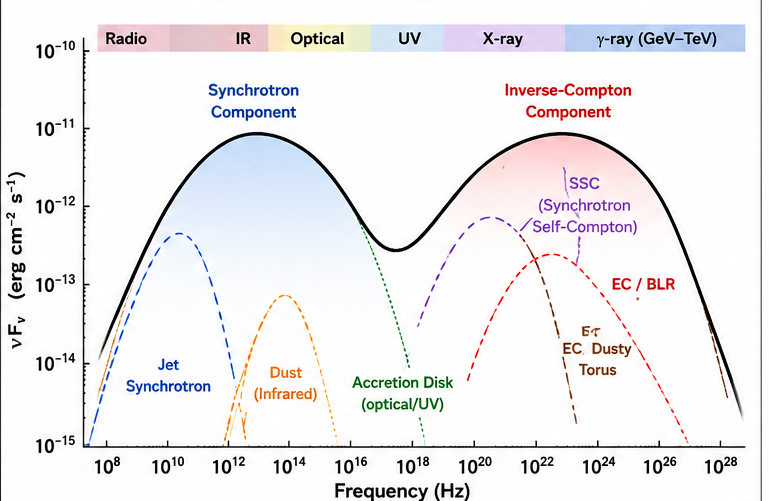
\includegraphics[width=\textwidth]{fig2_blazar_sed.png}
\caption{Schematic broadband SEDs illustrating the two principal blazar sub-populations. \textit{Left:} an FSRQ (low-synchrotron-peaked, LSP), in which the inverse-Compton peak substantially exceeds the synchrotron peak (high Compton dominance, $A_C \gg 1$), consistent with External Compton emission off disk, BLR, or torus photons. \textit{Right:} a high-synchrotron-peaked (HSP) BL~Lac object, in which the Compton peak is comparatively suppressed ($A_C \lesssim 1$), consistent with Synchrotron Self-Compton emission.}
\label{fig:sed}
\end{figure}

Figure~\ref{fig:sed} compares these two limiting cases schematically, motivating the leptonic sub-models discussed in Sections~3.3 and~3.4.

\subsection{Synchrotron Radiation}

The low-energy SED component is produced by optically thin synchrotron emission from ultrarelativistic electrons gyrating in the jet's magnetic field. For an electron population with a power-law energy distribution $N(\gamma) \propto \gamma^{-p}$, the resulting synchrotron spectrum follows $F_\nu \propto \nu^{-(p-1)/2}$ below the cooling break and steepens above it. The synchrotron peak frequency, $\nu_{pk}^{sy}$, depends on the magnetic field strength $B$, the Doppler factor $\delta$, and the characteristic electron Lorentz factor $\gamma_e$ as
\begin{equation}
\nu_{pk}^{sy} \propto \delta\, B\, \gamma_e^{2}.
\end{equation}
This peak frequency forms the basis of the LSP/ISP/HSP classification scheme and correlates strongly with Compton dominance and blazar subclass, tracing an underlying sequence in jet power, electron acceleration efficiency, and radiative cooling.

\subsection{Inverse Compton Scattering}

The high-energy SED component arises from inverse-Compton (IC) upscattering of lower-energy seed photons by the same relativistic electron population responsible for the synchrotron emission. In the Thomson regime, the scattered photon energy scales as $\varepsilon_{IC} \propto \gamma_e^{2}\, \varepsilon_{seed}$, so that the IC peak frequency tracks the synchrotron peak frequency scaled by $\gamma_e^2$. At sufficiently high seed-photon or electron energies, Klein--Nishina suppression reduces the scattering cross-section, softening and curving the resulting gamma-ray spectrum --- a mechanism frequently invoked to explain the spectral breaks observed near a few GeV in luminous FSRQs. The identity of the dominant seed photon field --- internal (jet synchrotron photons) or external (disk, BLR, torus) --- distinguishes the two principal leptonic emission models discussed below.

\subsection{Synchrotron Self-Compton Model}

In the Synchrotron Self-Compton (SSC) model, the seed photons for inverse-Compton scattering are the jet's own synchrotron photons. This mechanism is generally sufficient to reproduce the SEDs of BL Lac objects, which lack strong external radiation fields due to their radiatively inefficient accretion flows and weak or absent BLR emission. SSC models predict a tight correlation between the synchrotron and IC peak luminosities and frequencies, and are characterized by relatively low Compton dominance ($A_C \lesssim 1$), consistent with observations of BL Lac SEDs across the LSP--HSP sequence. Single-zone SSC models remain the standard baseline framework for HSP BL Lacs, though multi-zone or structured-jet extensions are sometimes required to reproduce fast VHE flaring (Figure~\ref{fig:ssc-ec}, left panel).

\subsection{External Compton Model}

\begin{figure}[htbp]
\centering
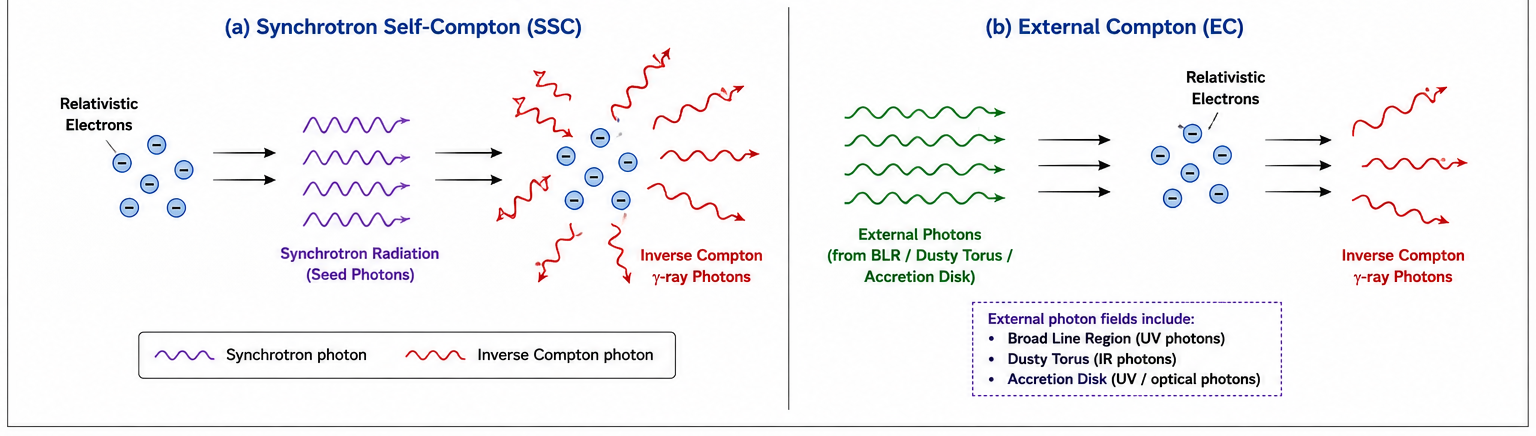
\includegraphics[width=\textwidth]{fig3_ssc_ec.png}
\caption{Schematic comparison of the two principal leptonic gamma-ray emission mechanisms. \textit{Left (SSC):} jet electrons upscatter their own synchrotron photons, requiring no external radiation field --- the dominant mechanism in BL~Lac objects. \textit{Right (EC):} jet electrons upscatter external seed photons supplied by the accretion disk, broad-line region, or dusty torus --- the dominant mechanism in FSRQs.}
\label{fig:ssc-ec}
\end{figure}

In the External Compton (EC) model, the dominant seed photons originate outside the jet --- from the accretion disk, the BLR, or the IR-emitting dusty torus. This mechanism is required to explain the high Compton dominance ($A_C \gg 1$) and soft, sharply curved gamma-ray spectra characteristic of powerful FSRQs, whose luminous, radiatively efficient accretion disks and dense BLR clouds provide copious external photon fields. EC scattering of infrared torus photons ($T_{\text{dust}} \sim 1000$~K) has proven particularly successful in reproducing the SEDs of high-redshift ($z > 2.5$) FSRQs, for which broadband modeling yields Doppler factors $\delta \sim 10$--$27$, magnetic fields $B \sim 0.10$--$1.74$~G, and compact emission-region sizes $R \le 0.05$~pc. The relative contribution of disk, BLR, and torus seed photons depends sensitively on the location of the emitting region within the jet, linking EC modeling directly to the unresolved question of the dissipation site.

\subsection{Hadronic Models}

Hadronic models attribute high-energy emission to relativistic protons co-accelerated alongside electrons in the jet. Gamma rays are produced either directly via proton synchrotron radiation or indirectly through photohadronic ($p\gamma$) interactions, which generate secondary electron--positron pairs and neutral- and charged-pion decay cascades. While hadronic and lepto-hadronic models remain viable, and in some cases favored, explanations for the SEDs of high-frequency-peaked BL Lac objects, pure hadronic scenarios applied to powerful FSRQs typically require jet kinetic powers of order $P_{jet} \sim 100$--$1000\, L_{\text{Edd}}$, exceeding plausible accretion-disk power budgets and standard jet-launching physics. Consequently, hadronic contributions are generally considered subdominant in FSRQs but remain an open and actively studied possibility in HSP BL Lacs, with direct observational support strengthened by multi-messenger neutrino associations (Section~5.1).

%%%%%%%%%%%%%%%%%%%%%%%%%%%%%%%%%%%%%%%%%%%%%%%%%%%%%%
\section{Variability of Blazars}

Flux variability across an enormous range of timescales --- from minutes to decades --- is among the most defining observational characteristics of blazars, reflecting the combined effects of relativistic beaming, shock propagation, magnetic reconnection, and underlying accretion-disk instabilities. Variability studies provide essential constraints on emission-region size, location, and the physical mechanisms driving particle acceleration.

\subsection{Short-term Variability}

Short-term (intraday to few-day) variability is most dramatically manifested in VHE gamma-ray flares with variability timescales as short as $t_v < 10$ minutes, as observed in sources such as Mrk~501, PKS~2155-304, and 3C~279. Causality arguments constrain the size of the emitting region according to
\begin{equation}
R \le \frac{\delta\, c\, t_v}{1+z},
\end{equation}
implying extremely compact dissipation zones and, in order to avoid catastrophic internal $\gamma\gamma \to e^{+}e^{-}$ pair-production opacity, exceptionally high Doppler factors ($\delta \sim 50$). Rapid variability is also commonly observed in X-rays (HSP BL Lacs) and in the optical/NIR bands, where minute-to-hour timescale flares are attributed to localized turbulent or reconnection-driven particle acceleration events within the jet, sometimes described by ``mini-jet'' or turbulent-cell models operating within a broader, more slowly varying emission region.

\subsection{Long-term Variability}

Long-term variability, probed via multi-year to multi-decade monitoring campaigns, reveals systematic trends and statistical properties that complement the transient, short-term picture. Approximately 80\% of blazars display a redder-when-brighter (RWB) spectral trend in the optical/NIR, consistent with variable red jet synchrotron emission increasingly dominating over a comparatively steady, bluer accretion-disk continuum as the source brightens. Cross-correlation analyses (e.g., using the z-transformed discrete correlation function) show that optical/NIR and gamma-ray variations are essentially co-spatial, with time lags consistent with zero (typically $<28$ days), while radio flares at 15~GHz lag gamma-ray activity by tens to hundreds of days due to opacity effects near the jet base. Statistically, FSRQs display systematically higher fractional variability ($F_{var} \sim 0.45$--$0.85$) than BL Lac objects ($F_{var} \sim 0.20$--$0.40$), power spectral density (PSD) slopes of $\alpha \sim 1.1$--$1.8$ indicative of pink-to-red noise processes, and flux distributions that are better described by log-normal than Gaussian statistics, pointing to multiplicative accretion-disk instabilities propagating into the jet. Multi-year searches for quasi-periodic oscillations (QPOs) using 12-year \textit{Fermi}-LAT light curves have identified candidate periodicities of 1.2--4 years in sources such as TXS~1902+556, S4~0814+42, and TXS~0518+211; however, global significances after trial-factor correction remain low ($\sim 0\sigma$), highlighting the difficulty of confirming true periodicity against a red-noise background.

%%%%%%%%%%%%%%%%%%%%%%%%%%%%%%%%%%%%%%%%%%%%%%%%%%%%%%
\section{Multi-Messenger Astronomy}

The advent of high-energy neutrino astronomy and gravitational-wave detection has opened new observational channels for probing the physical conditions within relativistic blazar jets, complementing traditional electromagnetic diagnostics and directly testing hadronic acceleration scenarios.

\subsection{Neutrino Observations}

Photohadronic ($p\gamma$) interactions within relativistic jets naturally produce high-energy neutrinos alongside gamma rays via charged-pion decay,
\begin{equation}
\pi^{+} \rightarrow \mu^{+} + \nu_\mu \rightarrow e^{+} + \nu_e + \bar{\nu}_\mu + \nu_\mu.
\end{equation}
The coincident detection of a high-energy IceCube neutrino event with a gamma-ray flare from the blazar TXS~0506+056 provided the first direct observational association between a blazar and a high-energy astrophysical neutrino, offering compelling evidence for hadronic particle acceleration and ultra-high-energy cosmic ray (UHECR) production within the jet. Subsequent archival and time-dependent analyses have searched for additional neutrino--blazar associations, and escaping UHECRs interacting with the extragalactic background light or cosmic microwave background can further generate non-variable, secondary TeV-scale gamma-ray emission observable independently of the primary flaring activity.

\subsection{Gravitational-wave Prospects}

While no gravitational-wave (GW) counterpart to blazar activity has yet been established, several theoretical channels motivate continued multi-messenger follow-up. Supermassive black hole binary systems, potentially hosted within or preceding the formation of blazar jets, are expected to produce low-frequency gravitational radiation detectable by pulsar timing arrays and, in the future, by space-based interferometers such as LISA; periodic or quasi-periodic blazar variability has occasionally been proposed, albeit speculatively, as an electromagnetic signature of such binary systems. More broadly, joint GW--electromagnetic--neutrino campaigns following the multi-messenger framework established for compact object mergers offer a template for future blazar studies, particularly as next-generation GW detectors improve sensitivity to potential precursor or associated high-energy electromagnetic activity from AGN environments.

%%%%%%%%%%%%%%%%%%%%%%%%%%%%%%%%%%%%%%%%%%%%%%%%%%%%%%
\section{Current Challenges}

Despite substantial observational and theoretical progress, several fundamental questions in blazar astrophysics remain unresolved. Foremost is the location of the gamma-ray dissipation region: whether flares originate deep within the sub-parsec BLR ($r < 0.1$~pc), where dense external photon fields favor efficient EC emission but risk severe $\gamma\gamma$ pair-production attenuation, or at parsec-scale distances ($r > 1$~pc) near the 43~GHz radio core, which avoids this attenuation but requires localized mechanisms such as turbulent magnetic reconnection to explain sub-hour variability across an otherwise extended jet cross-section. A second open issue concerns the persistent spectral breaks and logarithmic curvature observed near $\sim 2$~GeV in bright FSRQs such as 3C~454.3, for which competing explanations include Klein--Nishina suppression during EC scattering of BLR Lyman-$\alpha$ photons, $\gamma\gamma$ absorption by He~II/H~I Lyman continuum photons, intrinsic curvature in the electron energy distribution, and photon--axion-like particle (ALP) mixing. More broadly, the relative contributions of leptonic and hadronic processes, the reliability of candidate QPO detections against red-noise backgrounds, and the physical origin of rapid TeV variability all remain active areas of investigation.

%%%%%%%%%%%%%%%%%%%%%%%%%%%%%%%%%%%%%%%%%%%%%%%%%%%%%%
\section{Future Directions}

Continued progress in blazar astrophysics will be driven by next-generation facilities across the electromagnetic and multi-messenger spectrum. The Cherenkov Telescope Array (CTA) will deliver sub-minute temporal resolution and substantially improved VHE sensitivity, enabling tighter constraints on fast flares and on the EBL density at high redshift. X-ray polarimetry from \textit{IXPE}, complemented by prospective gamma-ray polarimetry missions, will directly measure jet magnetic field ordering and help discriminate between leptonic synchrotron/IC and hadronic emission scenarios. Expanded millimetric VLBI networks, including the Event Horizon Telescope, combined with time-dependent multi-frequency SED modeling, will enable near-real-time mapping of shock formation, jet precession, and magnetic reconnection sites at unprecedented angular resolution. Finally, the continued growth of neutrino telescopes (IceCube-Gen2, KM3NeT) and future gravitational-wave observatories will expand the multi-messenger reach of blazar studies, offering increasingly stringent tests of hadronic acceleration and jet-launching physics.

%%%%%%%%%%%%%%%%%%%%%%%%%%%%%%%%%%%%%%%%%%%%%%%%%%%%%%
\section{Conclusion}

Multiwavelength and multi-messenger observations, spanning radio to VHE gamma rays and extending to neutrinos, have transformed blazars into precision laboratories for studying relativistic jet physics, particle acceleration, and the coupling between accretion and outflow in supermassive black hole systems. The characteristic double-humped SED, well described by synchrotron and inverse-Compton processes within leptonic frameworks --- and, in select sources, supplemented by hadronic contributions --- together with rich phenomenology across short- and long-term variability, has enabled substantial progress in constraining jet composition, geometry, and energetics. Nonetheless, key questions concerning the location of gamma-ray dissipation, the origin of GeV spectral curvature, and the relative role of hadronic processes remain open. Forthcoming facilities in gamma-ray astronomy, high-energy polarimetry, ultra-high-resolution VLBI, and multi-messenger observation are poised to address these questions directly, securing blazars' continued importance at the forefront of high-energy astrophysics.

%%%%%%%%%%%%%%%%%%%%%%%%%%%%%%%%%%%%%%%%%%%%%%%%%%%%%%
% Bibliography: built directly into the document (no .bib file, no
% bibtex/biber run, and no external citation package required).
% This guarantees the document compiles in a single pdflatex pass
% on any standard LaTeX installation.
\begin{thebibliography}{99}

\bibitem{Urry1995}
C.~M.~Urry and P.~Padovani,
``Unified Schemes for Radio-Loud Active Galactic Nuclei,''
\textit{Publications of the Astronomical Society of the Pacific}, vol.~107, pp.~803--845, 1995.
doi:10.1086/133630

\bibitem{Blandford1978}
R.~D.~Blandford and M.~J.~Rees,
``Some comments on radiation mechanisms in Lacertids,''
\textit{Proceedings of the Pittsburgh Conference on BL Lac Objects}, pp.~328--341, 1978.

\bibitem{Atwood2009}
W.~B.~Atwood et al.,
``The Large Area Telescope on the Fermi Gamma-ray Space Telescope Mission,''
\textit{The Astrophysical Journal}, vol.~697, pp.~1071--1102, 2009.
doi:10.1088/0004-637X/697/2/1071

\bibitem{Gehrels2004}
N.~Gehrels et al.,
``The Swift Gamma-Ray Burst Mission,''
\textit{The Astrophysical Journal}, vol.~611, pp.~1005--1020, 2004.
doi:10.1086/422091

\bibitem{Harrison2013}
F.~A.~Harrison et al.,
``The Nuclear Spectroscopic Telescope Array (NuSTAR) High-Energy X-Ray Mission,''
\textit{The Astrophysical Journal}, vol.~770, p.~103, 2013.
doi:10.1088/0004-637X/770/2/103

\bibitem{Hinton2004}
J.~A.~Hinton,
``The Status of the H.E.S.S.\ Project,''
\textit{New Astronomy Reviews}, vol.~48, pp.~331--337, 2004.
doi:10.1016/j.newar.2003.12.004

\bibitem{Holder2006}
J.~Holder et al.,
``The First VERITAS Telescope,''
\textit{Astroparticle Physics}, vol.~25, pp.~391--401, 2006.
doi:10.1016/j.astropartphys.2006.04.002

\bibitem{Aleksic2016}
J.~Aleksi\'c et al.,
``The Major Upgrade of the MAGIC Telescopes,''
\textit{Astroparticle Physics}, vol.~72, pp.~76--94, 2016.
doi:10.1016/j.astropartphys.2015.04.004

\bibitem{Kormendy2013}
J.~Kormendy and L.~C.~Ho,
``Coevolution (Or Not) of Supermassive Black Holes and Host Galaxies,''
\textit{Annual Review of Astronomy and Astrophysics}, vol.~51, pp.~511--653, 2013.
doi:10.1146/annurev-astro-082708-101811

\end{thebibliography}

\end{document}